\documentclass[a4paper,man,natbib]{apa7}

\usepackage[english]{babel}
\usepackage[utf8x]{inputenc}
\usepackage{amsmath}
\usepackage{graphicx}
\usepackage[colorinlistoftodos]{todonotes}

% Added by me
\usepackage{lipsum}
\usepackage{float}
\usepackage{tikz}
\usepackage{tikz-qtree}
\usepackage{lscape}
\usepackage{multicol}
\usepackage{makecell}
\usepackage{array}
\usepackage{color, colortbl}
\usepackage{xr}
\externaldocument[sm-]{SM}
\newcolumntype{P}[1]{>{\centering\arraybackslash}m{#1}}
\newcommand{\YL}[1]{\textcolor{blue}{#1}}
\newcommand{\YLDEL}[1]{\sout{\textcolor{black}{#1}}}
%
\renewrobustcmd{\bfseries}{\fontseries{b}\selectfont}
\renewrobustcmd{\boldmath}{}
\newrobustcmd{\B}{\bfseries}
\title{Neural language models predict human acceptability errors in nested number agreement dependencies}
\shorttitle{NLMs predict acceptability errors}
\author{}
\affiliation{}

\abstract{Abstract}

\begin{document}
%\maketitle

% TEST
\section{Introduction}

According to a popular view in linguistics, the rich expressiveness
and open-ended nature of language rest on \emph{recursion}, the
possibly uniquely human ability to process nested structures \citep{Chomsky:1957, Hauser:etal:2002, Dehaene:etal:2015}. We
currently know very little about how such ability is implemented in
the brain, and consequently about its scope and limits.

In recent years, artificial neural-network models, rebranded as ``deep learning'' \citep{LeCun:etal:2015}, made tremendous advances in natural language processing \citep{Goldberg:2017}. Typically, neural networks are not provided with any explicit information regarding grammar or other types of linguistic knowledge. Neural Language Models (NLMs) are commonly initialized as ``tabula rasa'' and are solely trained to predict the next word in a sentence given its context \citep{Elman:1990}. Yet, these models achieve impressive performance, not far below that of humans, in tasks such as question answering or text summarization \citep{Radford:etal:2019}. Unlike their connectionist progenitors \citep{Rumelhart:etal:1986,Rumelhart:etal:1986b}, modern NLMs are not intended as cognitive models of human behaviour. They are instead developed to be deployed in applications such as translation systems or online content organizers. Still, NLMs' success in the practical natural language arena strongly suggests that they must infer non-trivial  linguistic knowledge from the raw data they are exposed to. % This has attracted the interest of linguists and cognitive scientists, curious to know  \textit{how} exactly NLMs handle grammatical structure \citep[see][for a survey]{Linzen:Baroni:2020}.

Given that it is easier to inspect the inner workings of NLMs than humans, we perform here an in-depth analysis of nested processing in NLMs. We uncover the neural circuitry they develop to handle it, and we use it to make predictions about human language processing. Importantly, we are not making claims about NLMs being models of the human brain. Rather, following \citet{McCloskey:1991}, we treat NLMs as a separate `animal species', whose way to address a linguistic task can provide insights into how the human brain might be tackling similar challenges.

Specifically, we explore multiple-structure nesting in the context of grammatical agreement. Long-distance agreement has traditionally been studied as one of the  best indices of online syntactic processing in humans, as it is ruled
by hierarchical structures rather than by the linear order of words in
a sentence \citep{Bock:Miller:1991, franck2002subject}. Consider for example the sentence: ``The \textbf{boys} under the \underline{tree} \textbf{know} the farmers'', where the number of the verb (`know') depends on its linearly distant subject (`boys'), and not on the immediately preceding noun `tree'.

Number agreement has also become a standard way to probe grammatical
generalization in NLMs \citep{Linzen:etal:2016,Bernardy:Lappin:2017,Giulianelli:etal:2018,Gulordava:etal:2018}. Very
recently, some steps were taken towards a mechanistic understanding of
how NLMs perform agreement. Specifically, \citet{lakretz2019emergence} showed that NLMs trained
on a large corpus of English developed a number-propagation mechanism for long-range dependencies. The core circuit of this mechanism is sparse, in the sense that it is comprised of an exceptionally small number of units (three out of 1300). This mechanism carries grammatical number information across various and challenging long-range dependencies, also in the presence of intervening nouns carrying opposite number.

The recursive power of language allows the construction of sentences with multiple nested agreement dependencies, as in: ``The \textbf{boys} that the \textit{father} under the \underline{tree} \textit{watches} \textbf{know} the farmers''. The mechanism we outlined above should be robust to the intervention of nested hierarchical structures, thus allowing correct percolation of number across the outermost long-distance agreement dependency (`boys/know'). However, the sparsity of the solution found by NLMs implies that only a number feature at a time can be tracked, thus predicting failure to handle \emph{embedded} dependencies within multiple nestings (`father/watches' in the example above). Intuitively, once the mechanism is ``filled'' by the outermost
dependency, it should not be able to track further number features.

We  start by confirming that the emergence of a sparse
agreement mechanism is a stable and robust phenomenon in NLMs by
replicating it with a new language (Italian) and grammatical feature
(gender). Next, we study how the sparsity of the agreement mechanism
affects recursive agreement processing, confirming our predictions
that the mechanism supports outermost agreement across nested
structures, but not multiple embedded agreements.

In the next part of the study, we treat our mechanistic understanding of
agreement in NLMs as an ``hypothesis generator''
\citep{Cichy:Kaiser:2019} about nested agreement processing in
humans. Suppose humans are also using a relatively small fraction of specialized units
to store and release agreement features across long-distance syntactic
structures. Then, we might observe a similar asymmetry in handling
outer- and innermost dependencies in recursive structures. We run a
behavioural experiment with Italian subjects to test this
hypothesis. The results are intriguing. One the one hand, humans do
not display the same dramatic failure to process embedded dependencies we observed in NLMs. However, they are indeed more prone to errors in embedded dependencies than in the longer-range outer ones, in accordance with our predictions. Moreover, a comparison between NLM and human results reveal overall remarkable similarity. 

We conclude that the NLM failed to discover a genuine mechanism for recursive processing of nested long-range agreements. However, our results also show how some degree of hierarchical processing can be performed by a device, such as the NLM, that did not develop full recursive capabilities. Furthermore, the similarity between the error patterns of humans and the model show that % that modern NLMs as compelling models for the study of language processing in humans, and our study shows how 
a detailed understanding of emergent mechanisms in NLMs can lead to formulating hypotheses about hierarchical structure processing that are relevant to human language parsing.


% We conclude by outlining future experiments that should allow to distinguish between two interpretations of the current data. According to one interpretation, humans' nested feature processing is radically different from the one emerging in NLMs, and genuinely capable of unbound recursive processing, limited only by finite resources. According to the other, humans' feature processing mechanism is akin to the one of NLMs, but only differs quantitatively. 

% Overall, our study illustrates how some degree of hierarchical processing can be performed by a device, such as an NLM, that did not develop full recursive capabilities. It also shows how a detailed understanding of emergent mechanisms in modern NLMs can lead to new and precise tests of human hierarchical structure processing.


%they also possess sophisticated backup mechanisms beyond the abilities developed by NLMs.


% \textbf{Earlier version of intro commented out below this line.}

% The prevailing view in linguistics suggests that the rich
% expressiveness and open-ended nature of human language require a
% computational ability to process nested tree structures, possibly
% unique to humans, which is based on
% \textit{recursion}. \citep{Chomsky:1957, Hauser:etal:2002,
%   Dehaene:etal:2015}. This view was developed in the context of the
% study of human linguistic \textit{competence}, which is described by a
% set of rules from which acceptable strings of a language can be
% generated. If a certain recursive construction can be generated from
% the grammar by the application of a rule, then a repeated application
% of the same rule could generate acceptable strings of an arbitrarily
% recursive complexity. In contrast, it is empirically established that
% human linguistic \textit{performance} is tightly limited in terms of
% processing complex nested constructions, due to various resource
% limitation, such as memory capacity or attention span \citep{}.

% In recent years, artificial neural-network models, rebranded as ``deep learning'' \citep{LeCun:etal:2015}, made tremendous advances in natural language processing \citep{Goldberg:2017}. Typically, neural networks are not provided with any explicit information regarding grammar or any type of linguistic knowledge. For example, Neural Language Models (NLMs) are commonly initialized as `tabula rasa' and are solely trained to predict the next word in the sentence given its context \citep{Elman:1990}. Yet, these models achieve an impressive performance not far below that of humans in tasks such as question answering or text summarization \citep{Radford:etal:2019}. This has naturally attracted recent interest into \textit{how} exactly these models perform the task, and the degree to which they infer genuine linguistic knowledge from raw data  \citep{}, with the ultimate hope that this will also provide insights into human language processing. 

% Grammatical agreement has traditionally been studied as one of the
% best indices of online syntactic processing in humans, as it is ruled
% by hierarchical structures rather than linear by the order of words in
% a sentence \citep{Bock:Miller:1991, franck2002subject}. Number
% agreement has also become a standard way to probe grammatical
% generalization in NLMs
% \citep{Linzen:etal:2016,Bernardy:Lappin:2017,Giulianelli:etal:2018,Gulordava:etal:2018}. Very
% recently, some steps were taken towards a mechanistic understanding of
% how NLMs perform agreement. Specifically, \citet{lakretz2019emergence} showed that NLMs trained
% on a large corpus of English developed a number-propagation mechanism for long-range dependencies. The core circuit of this mechanism is comprised of an exceptionally small number of units (three out of 1300). Despite its sparsity, this mechanism carries grammatical number information across various and challenging long-range dependencies, also in the presence of intervening nouns carrying opposite number. However, given the sparsity of the mechanism, it remains unclear how the network would
% process recursive structures having more than a single long-range
% dependency, such as in the case of multiple nested dependencies:
% Intuitively, once the mechanism is recruited by the outermost
% dependency, it is not able anymore to track the ones nested inside it.

% \dnote{I think this transition is difficult and doesn't do completely justice to what we do. Could we maybe add a few more sentences about recursion in networks? Or link it back to competence/performance again? It is important that the reader gets here the importance of what we try to do, I think it should sound less incremental than it sounds here.}
% In the present study, we start by investigating the recursive
% performance of NLMs, using number-agreement as a
% probe. We first confirm that the emergence of a sparse agreement mechanism is
% a stable and robust phenomenon in NLMs by replicating it with a new
% language (Italian) and grammatical feature (gender). Next, we study
% how the sparsity of the agreement mechanism affects recursive
% agreement processing, confirming our predictions that the mechanism
% strongly binds the depth of recursion. Finally, we test whether the
%  system we saw emerge in NLMs could serve as a
% model of recursion processing limitations in humans. The results of a
% behavioural study partly confirm our predictions, showing largely similar error patterns between NLMs and humans. 
% \YL{Add a sentence about differences}

% \textbf{Add boastful wrap-up sentence.}

\section{Number Agreement in Neural Language Models}

Neural language models have 

\begin{itemize}
    \item Describe previous results - a sparse mechanism for long-range number agreement
    \item Prediction to nested dependencies.
\end{itemize}

\begin{figure}
    \centering
    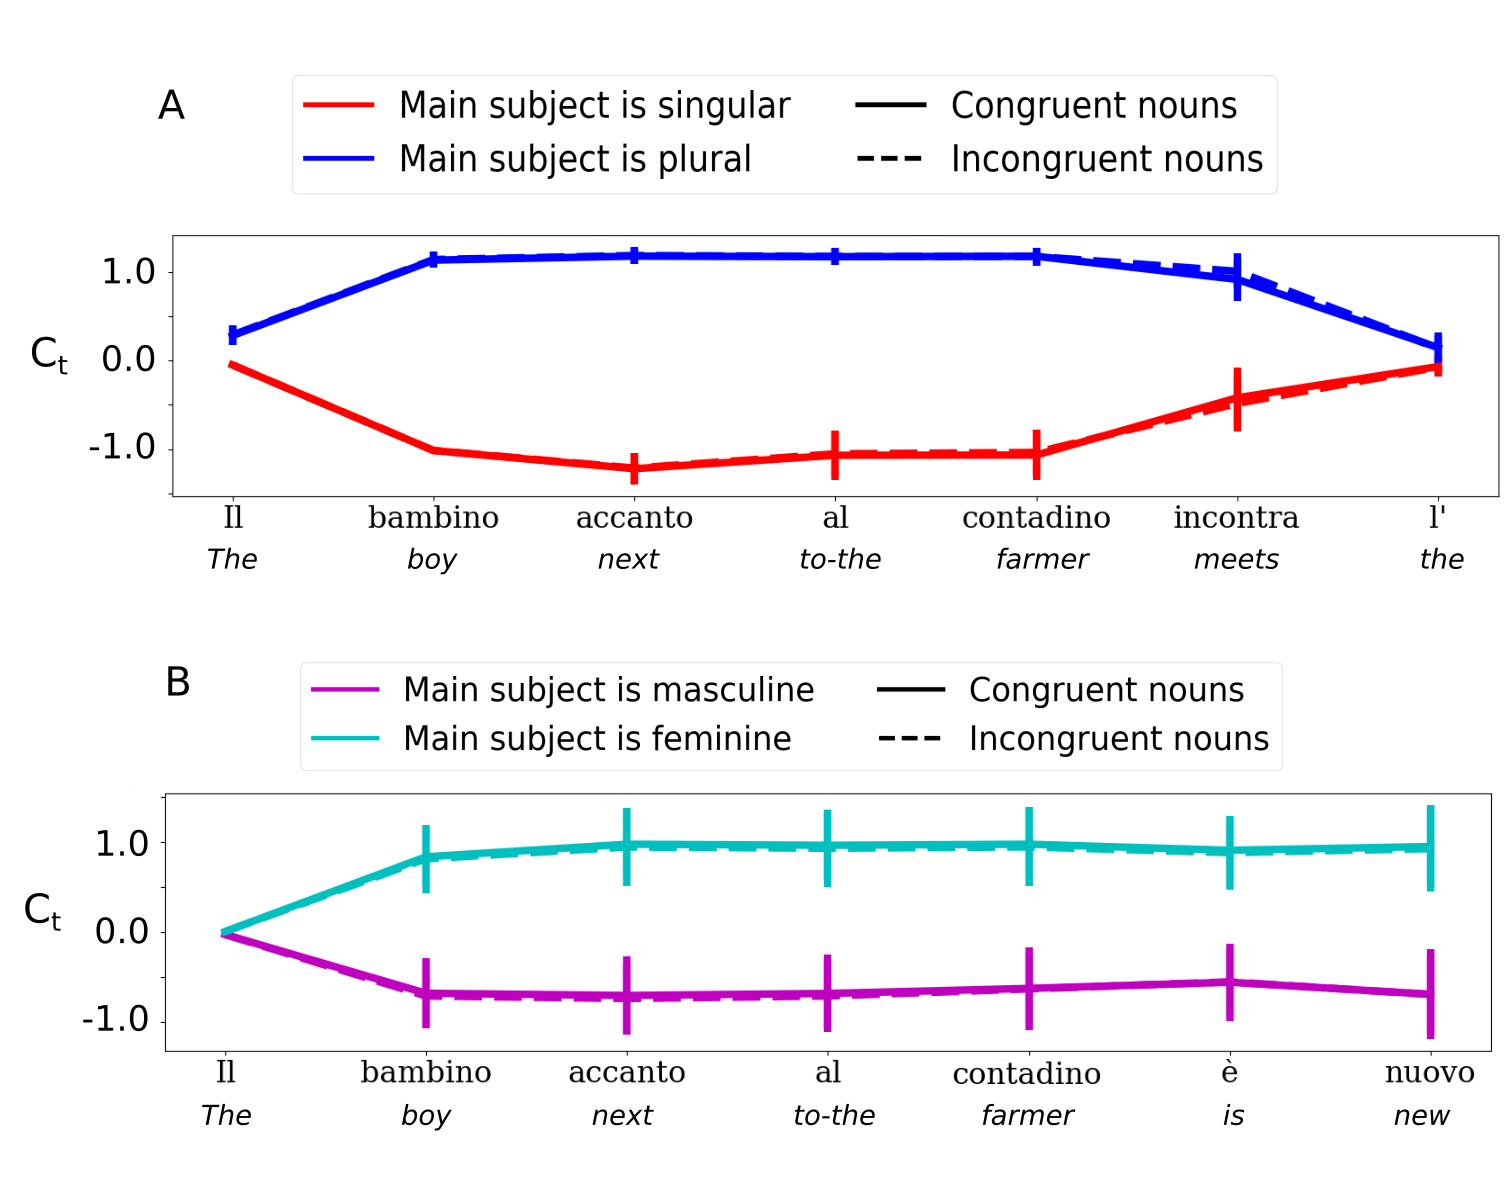
\includegraphics[width=\textwidth]{figures/model_activations_nounpp.png}
    \caption{\textbf{Cell activity of the number unit (panel A) and gender unit (panel B) during the processing of a single long-range dependency across a prepositional phrase:} four conditions are presented, corresponding to whether the main subject of the sentence is singular (red curves) or plural (blue), and to whether the main subject ('bambino') and the intervening noun ('contadino') have the same (congruent) or opposite number (incongruent)}
    \label{fig:nounpp}
\end{figure} 


\begin{figure*}
    \centering
    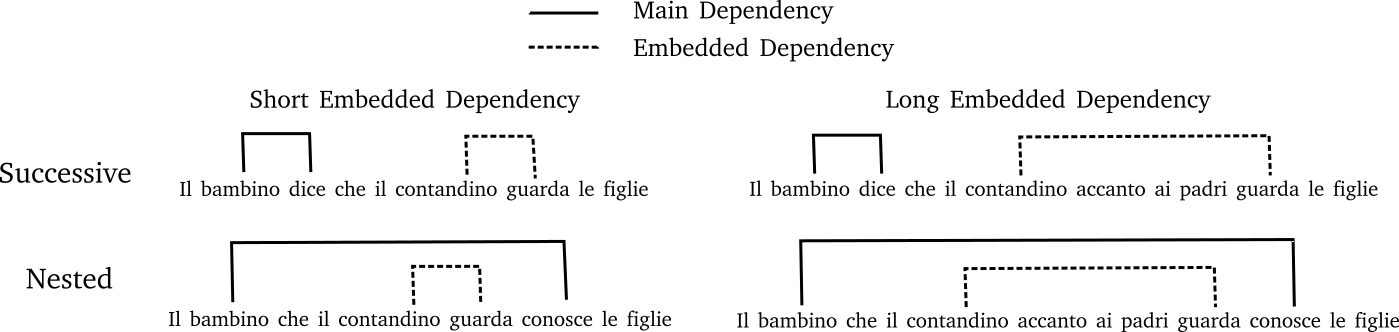
\includegraphics[width=\textwidth]{figures/design.png}
    \caption{\textbf{A full-factorial design for two subject-verb dependencies}. Human subjects and Neural Language Models (NLMs) were presented with sentences from four different syntactic structures, which all have two subject-verb dependencies: a main dependency (continuous lines) and an embedded dependency (dashed). The first factor of the design determines whether the two dependencies are \textit{successive} (top structures) or \textit{nested} (bottom), depending on whether the structure has a sentential complement (SC) or an object-extracted relative clause (objRC), respectively. The second factor determines whether the embedded dependency is \textit{short} (left side) or \textit{long} (right). We refer to the four resulting structures as: SC-short, SC-long, objRC-short and objRC-long.}
    \label{fig:design}
\end{figure*}
\section{Experimental Design}
To test the hypothesis that the sparsity of the long-range mechanism can lead to a significant processing difficulty at the embedded dependency, we created a two-by-two design that manipulates the above two conditions: (1) whether the two dependencies are \textit{successive} or \textit{nested}, and (2) whether the embedded dependency is \textit{short} or \textit{long} range. Figure \ref{fig:design} describes the resulting four NA-tasks: Short-Successive, Long-Successive, Short-Nested and Long-Nested ('Short' and 'Long' therefore refer to the length of the embedded dependency only).\footnote{\citet{Gulordava:etal:2018} made available several NLMs in several languages, whose hyperparameters were optimized by conducting an small grid search. 
These NLMs were since used in many subsequent studies \citep{Giulianelli:etal:2018, jumelet2019analysing, wilcox2018rnn, futrell2019neural}.
In our initial work \citep{lakretz2019emergence}, we explored the English NLM made available by this work, however, in this current work, we focused on the Italian NLM for two main reasons. \dnote{I'm a bit in doubt if this is the right place and way to mention we focus on a different language.}
First, we found that the overall performance of the Italian NLM was better on the more demanding nested construction. Second, in English, the plural is identical to the unmarked form of the verb, which also occurs as infinitive, in first and second person, and often as a noun. This makes the occurrence statistics unbalanced, in favor of plural.} 

The successive tasks serve as control, they minimally differ from the nested ones up to the embedded verb, by only a single word ('dice' ('says') in figure \ref{fig:design}). Note also that tasks that have a long embedded dependency have a third noun, which functions as a possible attractor inside the embedded dependency.

For each NA-task, we generated various \textit{conditions} by varying the number of the main and embedded noun, and of the attractor, Short-Successive and Short-Nested have each four conditions corresponding to the possible assignments of numbers to the main and embedded subjects - SS, SP, PS and PP. Similarly, Long-Successive and Long-Nested have eight conditions, based on the possible numbers of the main, embedded subject and attractor - SSS, SSP, SPS, etc. In what follows, by \textit{congruent subjects} we refer to conditions in which the main and embedded subjects share grammatical number (SS, PP, SSS, SSP, PPS and PPP), and by \textit{incongruent subjects} to the rest (SP, PS, SPS, etc.). By \textit{congruent attractor} we refer to conditions in which the embedded subject and the third noun share grammatical number (SSS, SPP, PSS and PPP), and by \textit{incongruent attractor} to conditions in which they differ (SSP, SPS, PSP, PPS) (Methods). 

To anticipate the results, we describe predictions specific for each task, and for each of its verbs, without currently specifying predictions for specific conditions (table \ref{tbl:predictions}): for Short- and Long-Successive, no significant processing difficulties are predicted on the main nor embedded verbs, since the long-range mechanism can in principle encode the grammatical number sequentially - once the long-range agreement mechanism finished processing the first dependency, its grammatical number can be removed from the long-range number units, before encoding the subsequent number of the embedded subject. For Short- and Long-Nested, the long-range mechanism is predicted to successfully process the main dependency and therefore no significant difficulties are predicted on the main verb (beyond the well-known relative difficulty to process center-embeddings, as reported for both humans \citep{traxler2002processing} and NLMs \citep{marvin2018targeted}). In contrast, the embedded dependency in Short-Nested cannot rely on the long-range agreement mechanism, as it is taken up in processing the main one, and therefore the processing of the embedded dependency can only rely on short-range mechanisms, which might not be as robust as the long-range one. To indicate the lack of clear prediction in this case, we mark both options in the table. Finally, in Long-Nested, the performance on the embedded verb is predicted to be significantly low, given that the long-range mechanism can process only a single agreement, as described above. 

\begin{center}
\begin{table}
\centering
\begin{tabular}{|P{3.5cm}||P{3.5cm}|P{3.5cm}|}
    \hline
    \B Sentence Type & \B Main Verb & \B Embedded Verb \\
    \hline
    Successive-Short & V  & V \\
    \hline
    Successive-Long & V & V \\
    \hline
    Nested-Short & V & - \\
    \hline
    Nested-Long & V & X \\
    \hline
\end{tabular}
\caption{A summary of the predictions of model performance on successive and nested dependencies based on the sparsity of the long-range mechanism. 'V' and 'X' represent high and low predicted performance on the agreement task, respectively. Due to possible compensation mechanisms carried by the short-range number units, we make no precise predictions regarding performance on the embedded verb of Nested-Short.}
\label{tbl:predictions}
\end{table}
\end{center}

\begin{figure*}
    \centering
    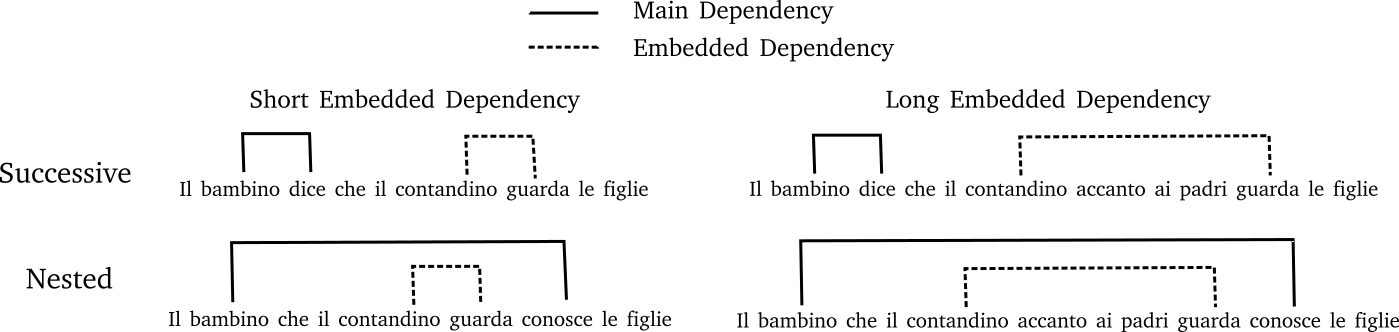
\includegraphics[width=\textwidth]{figures/design.png}
    \caption{\textbf{A full-factorial design for two subject-verb dependencies}. Human subjects and Neural Language Models (NLMs) were presented with sentences from four different syntactic structures, which all have two subject-verb dependencies: a main dependency (continuous lines) and an embedded dependency (dashed). The first factor of the design determines whether the two dependencies are \textit{successive} (top structures) or \textit{nested} (bottom), depending on whether the structure has a sentential complement (SC) or an object-extracted relative clause (objRC), respectively. The second factor determines whether the embedded dependency is \textit{short} (left side) or \textit{long} (right). We refer to the four resulting structures as: SC-short, SC-long, objRC-short and objRC-long.}
    \label{fig:design}
\end{figure*}

\section{Results}

\subsection{Nested Dependencies in Neural Language Models}

\subsubsection{Replication of previous results in Italian}
\paragraph{Ablation results}
\paragraph{Dynamics of the number unit} in nounpp
\begin{figure*}
    \centering
    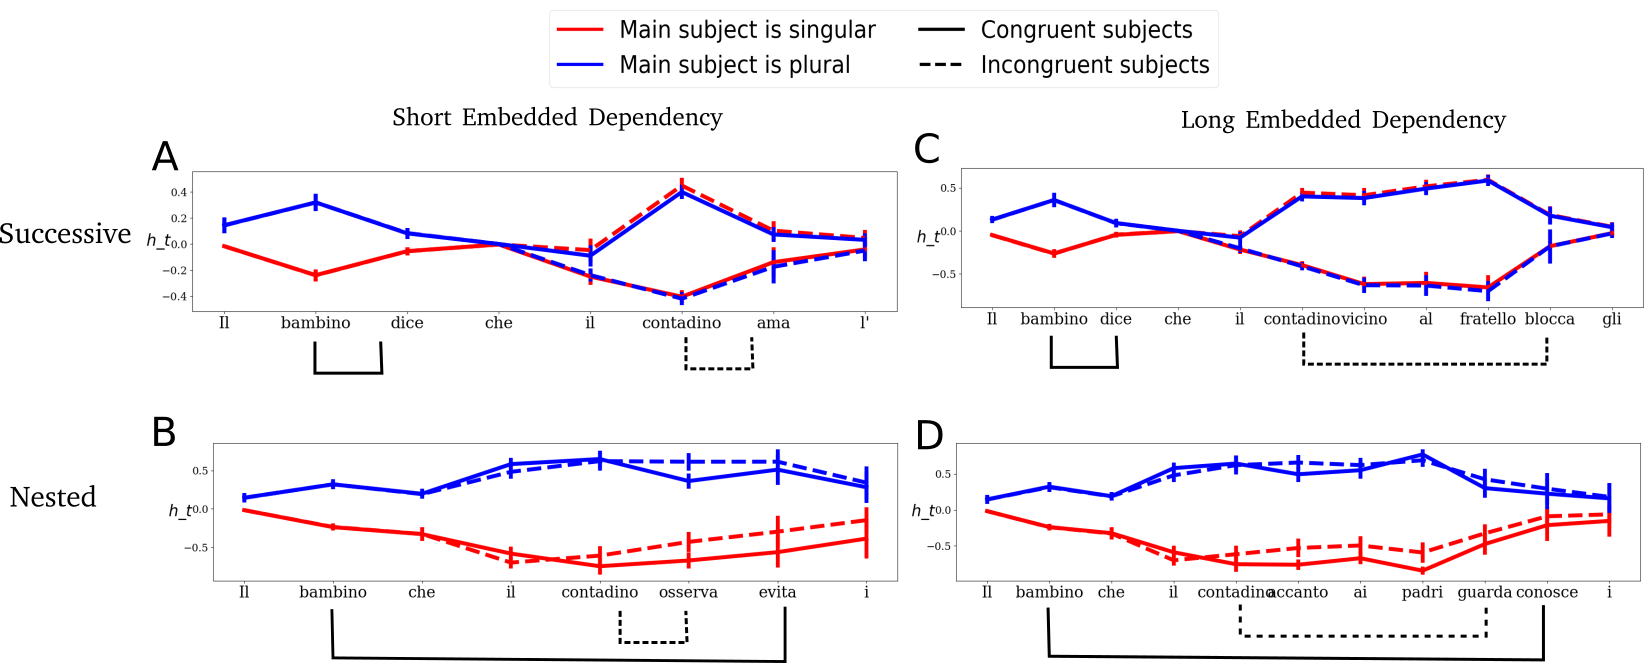
\includegraphics[width=\textwidth]{figures/model_activations.png}
    \caption{\textbf{Dynamics of the hidden activation of the number unit during the processing of two subject-verb dependencies.} Number-unit activity is presented for the four structures in the design: SC-short (panel A), SC-long (B), objRC-short (C) and objRC-long (D). For each structure, results are presented for the four conditions, corresponding to whether the main subject of the sentence is singular (red curves) or plural (blue), and to whether the main and embedded subjects have the same grammatical number (congruent; continuous lines) or not (incongruent; dashed lines).}
    \label{fig:my_label}
\end{figure*}



\subsubsection{The Processing of Nested Dependencies}


\begin{figure*}[h]
    \centering
    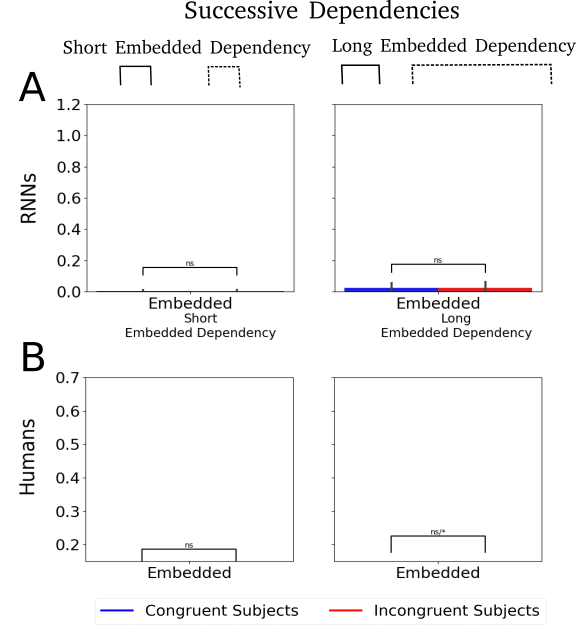
\includegraphics[width=10cm]{figures/error_rates_successive.png}
    \caption{\textbf{Error rates on the SC-short and SC-long structures:} collected from NLMs (panel A) and human subjects (B). Blue and red bars correspond to whether the main and embedded subjects agree on number (congruent subjects) or not (incongruent), respectively). Error bars represent standard error of the mean across all trials. ns - non significant.}
    \label{fig:my_label}
\end{figure*}


\begin{figure*}[h]
    \centering
    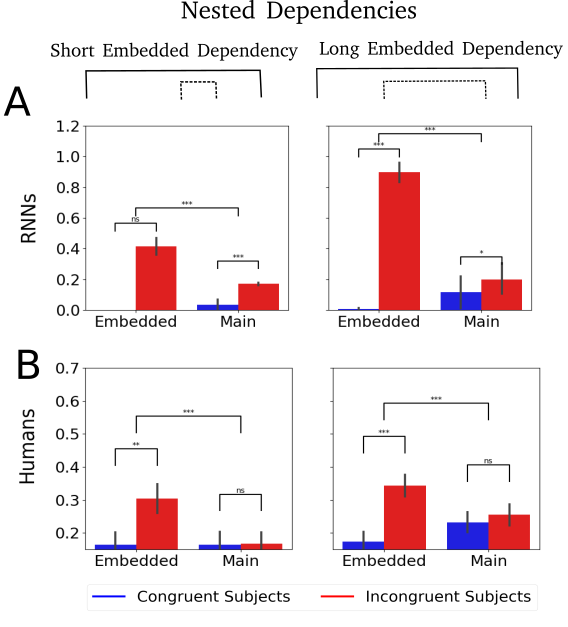
\includegraphics[width=10cm]{figures/error_rates_nested.png}
    \caption{\textbf{Error rates on the objRC-short and objRC-long structures:} collected from NLMs (panel A) and humans subjects (panel B). Blue and red bars correspond to whether the main and embedded subjects agree on number (congruent subjects) or not (incongruent), respectively. Error bars represent standard error of the mean across all trials. ns - non significant.}
    \label{fig:my_label}
\end{figure*}

% \lipsum[1]

\begin{table}[h]
\tiny
\centering
\parbox{.4\linewidth}{
\centering
    \begin{tabular}{ |P{3cm}|P{1.3cm}|P{1.3cm}|  }
    \hline
    \rowcolor{cyan}
    \multicolumn{3}{|c|}{\textbf{Short-Successive}} \\
    \hline
    \rowcolor{cyan}
    \textbf{Effect} & \textbf{Humans} & \textbf{RNNs} \\
    \Xhline{3\arrayrulewidth}
    \rowcolor{green}
    \textbf{Subject Congruence (Embedded verb)} & X & X \\
    \hline
    
    \end{tabular}
}
\hfill
\parbox{.4\linewidth}{
\centering
    \begin{tabular}{ |P{3cm}|P{1.3cm}|P{1.3cm}|  }
    \hline
    \rowcolor{cyan}
    \multicolumn{3}{|c|}{\textbf{Long-Successive}} \\
    \hline
    \rowcolor{cyan}
    \textbf{Effect} & \textbf{Humans} & \textbf{RNNs} \\
    \Xhline{3\arrayrulewidth}
    \rowcolor{green}
    \textbf{Subject Congruence (Embedded verb)} & X & X \\
    \hline
    
    \end{tabular}
}

\vspace{25pt}

\parbox{.4\linewidth}{
\centering
    \begin{tabular}{ |P{3cm}|P{1.3cm}|P{1.3cm}|  }
    \hline
    \rowcolor{cyan}
    \multicolumn{3}{|c|}{\textbf{Short-Nested}} \\
    \hline
    \rowcolor{cyan}
    \textbf{Effect} & \textbf{Humans} & \textbf{RNNs} \\
    \Xhline{3\arrayrulewidth}
    \rowcolor{magenta}
    \textbf{Subject Congruence (Main verb)} & X &  V\\
    \Xhline{3\arrayrulewidth}
    \rowcolor{green}
    \textbf{Subject Congruence (Embedded verb)} & V &  V\\
    \hline
    \rowcolor{green}
    \textbf{Interaction: Subject-Congruence Verb-Position} & V &  V\\
    \hline
    
    \end{tabular}
}
\hfill
\parbox{.4\linewidth}{
\centering
    \begin{tabular}{ |P{3cm}|P{1.3cm}|P{1.3cm}|  }
    \hline
    \rowcolor{cyan}
    \multicolumn{3}{|c|}{\textbf{Long-Nested}} \\
    \hline
    \rowcolor{cyan}
    \textbf{Effect} & \textbf{Humans} & \textbf{RNNs} \\
    \Xhline{3\arrayrulewidth}
    \rowcolor{magenta}
    \textbf{Subject Congruence (Main verb)} & X &  V\\
    \Xhline{3\arrayrulewidth}
    \rowcolor{green}
    \textbf{Subject Congruence (Embedded verb)} & V &  V\\
    \hline
    \rowcolor{green}
    \textbf{Interaction: Subject-Congruence Verb-Position} & V &  V\\
    \hline
    
    \end{tabular}
}
\caption{A summary of all effects  humans and RNNs.}
\label{tbl:comparison}
\end{table}

\section{Materials and Methods}

\subsection{NA-tasks}

For both our ablation and nestedness experiments \dnote{do we have a name for this? I know it is not ``nestedness-experiments'', but I needed a way to refer to them in both the text and the tables.} we two and four different \emph{number-agreement (NA)} tasks, respectively.
We give a short description of these tasks below, an overview can be found in Table~\ref{tab:na-tasks-overview}.
The complete lexicon we used to generate all stimuli can be found in the supplementary materials, Table~\ref{}.

\subsubsection{Ablation experiments}
For our ablation studies, which we conduct to replicate and extend the findings of \citet{lakretz2019emergence} to Italian, we use two different types of NA tasks.

\paragraph{NounPP}
First, to establish the presence of long-range \emph{number} units, we create an Italian version of \citeauthor{lakretz2019emergence}'s \citeyear{lakretz2019emergence} NounPP task.
This data set consists of 4000 sentences in which the subject is separated from the main verb by a prepositional phrase.
I.e., an example of a sentence in this dataset, which we dub \emph{nounPP}, is ``il \textbf{ragazzo} accanto alla \underline{donna} \textbf{conosce} \ldots'' (the \textbf{boy} next to the \underline{woman} \textbf{knows}).
We systematically vary the number of both the subject and the noun in the prepositional phrase (also referred to with the term \emph{attractor}), resulting in four different conditions: singular-singular (SS), singular-plural (SP), plural-singular (PS) and plural-plural (PP).
For all of these conditions, we generate 1000 sentences by randomly sampling (object and subject) nouns, verbs and prepositions from a list of options, reported in Table \ref{}.
\dieuwke{Should we say something about ensuring that sentences are at least somewhat semantically acceptable, i.e. excluding sentences like ``Il figlio sotto il cane \ldots''}

\paragraph{NounPP-gender}
To investigate if the model has long-range \emph{gender} units, we adapt the NounPP task to end with a predicative adjective.
For example: ``il \textbf{ragazzo} accanto alla \underline{donna} \`{e} \textbf{basso} (the \textbf{boy} next to the \underline{woman} is \textbf{short}).
In this NA-task, which we call \emph{NounPP-gender}, we focus on the adjective, which in Italian should match both the number and the gender of the subject.
We again consider four different conditions: feminine-feminine (FF), feminine-masculine (FM) masculine-feminine (MF) and masculine-masculine (MM), within which the number of the subject and attractor is ranomly varied.
Similar to the NounPP task, we sample 1000 sentences per condition, using the word lists provided in Table~\ref{}.

\subsubsection{Nested experiments}

\dieuwke{April 30 -- I'll continue with this tomorrow}


\begin{table}[h!]
    \setlength\tabcolsep{2mm}
\small
\centering
\begin{tabular}{lll}
\multicolumn{3}{c}{\centering \textit{Probing number/gender units}}\\
\hline
\hline
\emph{Nounpp} & \texttt{\textbf{NP$_a$} prep NP$_b$ \emph{V$_a$}} & \specialcell{Il \textbf{ragazzo} accanto alla \underline{donna} \textbf{conosce}\vspace{-3mm}\\({\scriptsize The \textbf{boy} next to the \underline{woman} \emph{knows}})} \\
\emph{Nounpp-gender} & \texttt{\textbf{NP$_a$} prep NP$_b$ BE$_a$ \emph{ADJ$_a$}} & \specialcell{Il \textbf{ragazzo} accanto alla \underline{donna} \`{e} \textbf{basso}\vspace{-3mm}\\({\scriptsize The \textbf{boy} next to the \underline{woman} is \textbf{short}})}\\
~\\
\multicolumn{3}{c}{\centering \textit{Nesting experiments}}\\
\hline
\hline
\emph{Short-Successive} & \texttt{NP$_a$ V$_a$ che NP$_b$ V$_b$} & \specialcell{Il \textbf{figlio} \textbf{dice} che il \emph{ragazzo} \emph{ama}\vspace{-3mm}\\{\scriptsize The \textbf{son} \textbf{says} that the \emph{boy} \emph{loves}}} \\
\emph{Long-Successive} & \texttt{NP$_a$ V$_a$ che NP$_b$ P NP$_c$ V$_b$} & \specialcell{Il \textbf{figlio dice} che l'\emph{amico} accanto al \underline{ragazzo} \emph{conosce}\vspace{-3mm}\\{\scriptsize The \textbf{son says} that the \emph{friend} next to the \underline{boy} \emph{knows}}} \\
\emph{Short-nested} & \texttt{NP$_a$ che NP$_b$ V$_b$ V$_a$ } & \specialcell{Il \textbf{figlio} che il \emph{ragazzo} \emph{osserva} \textbf{evita}\vspace{-3mm}\\{\scriptsize The \textbf{son} that the \emph{boy} \emph{observes} \textbf{avoids}}} \\
\emph{Long-nested} & \texttt{NP$_a$ che NP$_b$ P NP$_c$ V$_b$ V$_a$} & \specialcell{Il \textbf{figlio} che la \emph{ragazza} accanto ai \underline{padri} \emph{ama} \textbf{evita}\vspace{-3mm}\\{\scriptsize The \textbf{son} that the \emph{girl} next to the \underline{fathers} \emph{loves} \textbf{avoids}}} \\
\end{tabular}
\caption{\textbf{The NA-tasks we use for our ablation and nesting experiments.}
The first column denotes the name of the task.
The second column indicates the format of the sentences, where \texttt{NP} is used as an abbreviation of \texttt{Det N}.
The indices $a$, $b$ help identify the noun-verb relationships in the templates.
I.e. in the \emph{long-nested} condition condition, there are three nouns and two verbs, the indices $a$ and $b$ indicate that the last verb \texttt{V$_a$} is syntactically dependent on the first noun phrase \texttt{NP$_a$}, whereas the penultimate verb \texttt{V$_b$} instead should match the features of the second noun phrase \texttt{NP$_b$}.
Note that for the long- and short-nested conditions, we test both the \emph{inner} verb \texttt{V$_b$} and the \emph{outer} verb \texttt{V$_a$}.
The third and last column contains an example of a sentence in the NA-task, along with its English translation.
Bold and italic face show the relations indicated by the indices in the templates.
For every NA-task, we systematically vary the \emph{number} (and in the gender-case also gender) of all nouns in the template, resulting in four different conditions (SS, SP, PS and PP) for the NA-tasks with two nouns (\emph{Nounpp}, \emph{Nounpp-gender}, \emph{Short-successive} and \emph{Short-nested}) and eight different conditions (SSS, SSP, SPS, SPP, PSS, PSP, PPS and PPP) for the NA-tasks with three nouns (\emph{Long-succesive} and \emph{Long-nested}).
The examples shown are all SS and SSS conditions.
\textbf{M: I agree that it might be a good idea to use NP, however this should also apply to the gender case \dieuwke{D: done}. Also, indexing is nice, but it should be used thoroughly \dieuwke{better like this?}. Also, it should also be shown in the examples. On the other hand, I am not sure of why only one noun/verb is capitalized/italicized for short- and long-nested, given that we test both main and embedded (perhaps, worth duplicating these cases?). \dieuwke{better like this?}}}\label{tab:na-tasks-overview}
\end{table}

\subsection{Behavioral Experiment}
\subsubsection{Participants}
61 psychology students from the University of Milano-Bicocca (males = XX; Age = XX ± XX; Education = XX ± XX) took part in the experiment in exchange of course credits. Participants were Italian native speakers and were naive with respect to the experiment purpose. The study was approved by the ethical committee of the Department of Psychology, and ethical treatment was in accordance with the principles stated in the Declaration of Helsinki.

\subsubsection{Stimuli}
Stimuli comprised i) acceptable sentences; ii) violation trials, containing a number violation on the verb of one of the subject-verb agreements; iii) filler sentences, comprising several syntactic and semantic violations. 

Acceptable sentences were created using a pool of 10 nouns, 19 verbs, 4 prepositions (see table S1).
Starting from this pool of sentences, number-violation and filler trials were created by replacing either the main or embedded verb by the opposite form of the verb with respect to number. For example, ``il fratello che lo studente *accolgono ama i contadini'' (``the brother that the student *welcome loves the farmers'').

Filler trials contained either semantic violations or a syntactic violation that does not concern number. Syntactic violations were generated by either i) replacing a verb with a wrong person without changing number, for example: ``il fratello che lo studente *accolgo ama i contadini'' (``the brother that the student *welcome-1st-pers-sing loves the farmers''); or ii) replacing a verb with a noun, for example, ``il fratello che lo studente *amica ama i contadini'' (``the brother that the student *friend loves the farmers''; note that the chosen replacement nouns were not ambiguous with verb forms in Italian); or iii) replacing a verb with its infinitive form, for example, ``il fratello che lo studente *accogliere ama i contadini'' (``the brother that the student *to-welcome loves the farmers''). Semantic violations were generated by either replacing one of the nouns with i) an inappropriate abstract one, for example, ``la *filosofia dice che la figlia ama la madre'' (``*philosophy says that the daughter loves the mother''); ii) or an inanimate noun, for example, ``la *matita dice che la figlia ama la madre'' (``the *pencil says that the daughter loves the mother''). To avoid correlation between abstract or inanimate nouns and semantic violations, half of these filler trials were felicitous, for example, ``il padre dice che la figlia ama la *filosofia'' (``the father says that the daughter loves *philosophy''), or ``il padre dice che la *matita appartiene alla figlia'' (``the father says that the *pencil belongs to the daughter''). See Supplementary Materials for more details.

In total, 540 sentences were presented to each participant, randomly sampled from a larger pool. Of these, 180 sentences were acceptable, 180 had a number violation, and 180 were fillers.

\subsubsection{Paradigm}
The experiment was conducted in two sessions of 270 trials each, which were performed by participants in different days. Each session lasted around 45 minutes. The two sessions took place at the same time of the day at a maximum temporal distance of two weeks. After receiving information about the experimental procedure, participants were asked to sign a written informed consent. 

Stimuli were presented on a 17” computer screen in a light-grey, 30-point Courier New font on a dark background. Sentences were presented using Rapid Serial Visual Presentation (RSVP). Each trial started with a fixation cross appearing at the center of the screen for 600 ms, then single words were presented with SOA=500 ms, 250 ms presentation followed by 250 ms of black screen. At the end of each sentence, a blank screen was presented for 1500 ms, then a response panel appeared, with two labels “correct” and “incorrect”, on two sides of the screen (in random order each time) for a maximal duration of 1500 ms. A final screen, showing accuracy feedback was presented for 500 ms.

Participants were informed that they would be presented with a list of sentences which could be acceptable or containing a syntactic or semantic violation. They were instructed to press the “M” key of the Italian keyboard as fast as possible once they detected a violation. Sentences were presented up to their end even when participants pressed the button earlier. Then, in the response panel, participants were asked to press the “X” key if the sentence was correct, or “M” when the sentence was not correct. During the entire session, participants were asked to keep their left index over “X” and their right index over “M”. After each trial, participants received feedback concerning their response: ``Bravo!'' (``Good!'') in  case the sentence was correct, ``Peccato..'' (i.e. ``too bad...'') when it was incorrect. \textbf{M: Rather than the sentence, the response?} At the beginning of each session, participants performed a training block comprising XX items. The training section included all types of stimuli.

\subsubsection{Data and Statistical Analyses}
In ungrammatical trials, a violation could occur on either the main or embedded verb. Errors therefore correspond to trials in which a violation was missed. Since in ungrammatical trials a violation occurred on only one of the two verbs, the error can be associated with either the main or embedded dependency. In grammatical trials, errors correspond to trials in which participants reported a violation despite its absence. In contrast to ungrammatical trials, in which the violation marks the dependency, in grammatical trials it is not possible to associate an error with one of the two dependencies. Moreover, due to the presence of filler trials, the false detection of a violation could be unrelated to grammatical agreement (for example, a false detection of a semantic violation). Agreement errors were therefore estimated from ungrammatical trials only.

Statistical analyses were carried out using R, an open-source programming language \citep{R}. For each hypothesis to be tested, we fitted a mixed-effects logistic regression model \citep{Jaeger2008}, with participant and item as random factors, using the lme4 package for linear mixed effects models \citep{Bates}. Following \citet{Baayen:etal:2008}, we report the results from the model with the maximal random-effects structure that converged for all experiments. 
%Data from participants with accuracy below 0.8 on the filler items were excluded from analyses.

\subsection{Language Model}
\subsubsection{Model Description}
We use the Italian NLM made available by \citet{Gulordava:etal:2018} at \url{https://github.com/facebookresearch/colorlessgreenRNNs}.
It consists of two layers with 650 Long-Short Term Memory (LSTM) units \citep{Hochreiter:Schmidhuber:1997}, input and output embedding layers of 650 units and input and output layers of size 50000 (the size of the vocabulary). The weights of the input and output embedding layers are not shared.
The last layer of the model is a softmax layer, whose activations sum up to 1 and as such corresponds to a probability distribution over all words in the NLM's vocabulary. The model was trained on a dump of the Italian Wikipedia (80M word token, 50K word types). See  \citet{Gulordava:etal:2018} for further details.

\subsubsection{Control model Training} 
\textbf{M: Given how little emphasis this has in the main text, how about moving it to supplementary?} In addition to the NLM made available by \citet{Gulordava:etal:2018}, we train an additional 19 models using the same procedure and corpus (drawn from Wikipedia), giving 20 models in total. 
The models differ in the order in which those sentences are presented as well as the initialization of their weights.
For all runs, we use a learning rate of 20, a batch size of 64 and a dropout rate of 0.2, the hyperparameters that \citet{Gulordava:etal:2018} reported to work best for this particular corpus and setup.
Following Gulordava, but contrary to common practice in language modeling, we train the models on separate sentences, rather than longer pieces of discourse.
As common practice for training language models, we do not use an optimizer, but instead use a \emph{plateau-based} learning scheme, in which we half the learning rate whenever the validation perplexity of the model reaches a plateau.

\subsubsection{Model Evaluation} After training, we evaluate the resulting 20 models by considering their perplexity on a shared test set\footnote{\url{https://dl.fbaipublicfiles.com/colorless-green-rnns/training-data/Italian/test.txt}}. For the NA-tasks, following \citet{Linzen:etal:2016}, we compute accuracy by presenting the preamble of each sentence to the NLM and then compare the output probabilities assigned to the plural and singular forms of the verb.\textbf{How about the gender experiment?} On each sentence, the model is scored 1 if the probability of the correct verb is higher than the wrong, and else 0. Model accuracy is then defined as the average of these scores across all sentences in the NA-task. \textbf{M: I think it would be better to only refer here to evaluation of the main model.}

\subsubsection{Ablation Experiments}
To identify units that play an important role in the encoding of number and gender, we run a series of ablation tests.
In these ablation tests, we assess the impact of a \emph{single unit} on model performance by setting the activation of the unit to zero and then recomputing the performance of the model on the Noun-PP NA-task. \textbf{M: consistency in how the tasks are called: Noun-PP, Nounpp, NounPP\ldots} 
We conduct such ablation studies for all recurrent units in the network, resulting in 1300 ablation studies per model.


\section{General Discussion}
% Re-iteration on the motivations and goals
We investigated how recursive processing of number agreement is performed by Neural Language Models (NLMs), treating them as `hypothesis generators' for understanding human natural-language processing. To this end, we contrasted how NLMs process successive and nested constructions, and tested resulting predictions about human performance. 

% Summary of the results on a single dependency in NLMs
\subsection{A Sparse Agreement Mechanism Consistently Emerges in NLMs Across Languages and Grammatical Features}
Using number-agreement tasks with a single subject-verb dependency, we first replicated in Italian previous findings reported for an English NLM, and extended these findings to another grammatical feature, namely, gender. We found that for both number and gender agreement a sparse mechanism emerged in an Italian NLM during training. These findings suggest that the emergence of a sparse agreement mechanism in NLM is a robust phenomenon across languages and grammatical features. 

The results are moreover consistent with the recent finding that a sparse agreement mechanism emerged in an NLM trained on an artificial language having deep nested structures (i.e., with more than two levels of nesting), suggesting that the sparsity property is not due to the rare occurrence of deep nested structures in natural language \citep{lakretz2020recursion}. 

The sparsity and specificity of the agreement mechanism suggests that NLMs develop a separate `module' for at least one specific kind of grammatical processing. This is in contrast with semantic information, that NLMs pack into dense embedding vectors, supporting the computation of graded similarity relations \citep{Mikolov:etal:2013a,Jurafsky:Martin:2020}.

% While grammatical information pertinent to agreement is encoded by a small number of syntax and long-range feature units, non-grammatical information, such as semantic information, is high-dimensional, encompassing complex similarity relations among items, and thus benefitting from rather distributed encoding across many units. Indeed, NLMs commonly develop dense representations for the processing of semantic information, by mapping discrete symbols from the lexicon to continuous vectors in a relatively low-dimensional space, determined by the input embedding layer (Materials and Methods). Sparsity and specificity of the agreement mechanism in NLMs therefore suggests the separate processing of grammatical and semantic information in the network.

It is an open question whether semantic and syntactic information is encoded and processed jointly or separately in the `language network' of the human brain \citep{pallier2011cortical}. It was traditionally assumed that syntactic processing takes place in localized brain regions, such as Broca's area \citep[e.g.,][]{dapretto1999form}. However, some recent studies cast doubt on this view, providing evidence that semantic and syntactic processing in the language network cannot be dissociated from one another \citep{mollica2018high, siegelman2019attempt, fedorenko2020lack}. There are clearly substantial differences between the human brain and NLMs. However, our findings suggest that separating syntactic from semantic processing is computationally advantageous for addressing the language-modeling task \citep[][for related studies.]{ullman2004contributions, o2006biologically, russin2019reilly} 

% Summary of the results on two dependencies in NLMs
\subsection{Processing of Nested Dependencies in Humans and NLMs}
We next explored agreement processing of recursive structures that comprise a subject-verb dependency nested within another one. We first confirmed the prediction stemming from the sparsity of the NLM agreement mechanism. The network exhibits exceptional difficulty in processing an embedded long-range dependency within a nested construction. Since NLMs lack a recursive procedure to handle multiple dependencies, once the number units are taken up for the encoding of the outermost dependency, the network fails to process an embedded long-range dependency. In contrast, we found that NLMs achieve relatively good performance on processing \textit{short-range} embedded dependencies, as they can rely on short-range number units outside the core sparse mechanism. The cooperation between the long- and short-range mechanisms in NLMs therefore allows the network to support the processing of a large proportion of agreement constructions in natural language, failing substantially on only relatively uncommon constructions, having two or more nested dependencies that are all long-range. \textbf{M: I like the story about such constructions being relatively uncommon: but do we know that they are? If not, we should perhaps make it clear that it is our conjecture that such constructions are relatively uncommon.}

Human results were found to have both similarities with the agreement-error patterns of NLMs and several important points of discrepancy:

\subsubsection{Main Similarities}
\begin{itemize}
    \item \textbf{Low error-rates on successive dependencies}: humans and the NLM made a relatively small number of agreement errors on the embedded verb of successive dependencies. For NLMs, this is in accordance with the sequential processing observed in its dynamics (Figure \ref{fig:2by2_dynamics}). The agreement mechanism resets after the first dependency and is thus available to process the second one. For humans, these findings are in accordance with the relatively good performance of humans on right-branching constructions.
    \item \textbf{Subject-congruence effect in nested constructions}: in the case of a plural subject attractor, for all verbs, both humans and NLMs made significantly more errors in incongruent cases, in which the main and embedded subjects had opposite grammatical numbers.
    \item \textbf{Higher error-rate on embedded compared to main verbs of nested dependencies}: a positive interaction between verb position and subject congruence was found for both short- and long-range embedded dependencies, suggesting that embedded verbs are more error prone, confirming \textit{Prediction 1}.

    
\end{itemize}

\subsubsection{Main Differences}
    \begin{itemize}
        \item \textbf{NLM performance is worse than chance level on the embedded verb of Long-Nested}: the major difference between NLM and human performance (Figures \ref{fig:error_rates_plural_subject}\&\ref{fig:error_rates_all_conditions}) lies in the behaviour of the NLM with respect to the embedded verb in Long-Nested. The NLM was worse than chance level, meaning that in most trials the network predicts the grammatical number of the embedded verb based on the number of the main subject, which is encoded and carried through by the agreement mechanism. In contrast, human performance is better than chance level (although only marginally so, $p = 0.028$).
        \item \textbf{Prediction 2 was not confirmed in humans}: the NLM made significantly more errors on the embedded dependency when the dependency was long-range. This was not confirmed in humans, where the interaction between subject-congruence and length of embedded dependency was not significant. Humans as well, however, made more errors in the long-range case.
        \item \textbf{Absence of markedness effect in the NLM}: while humans made more agreement errors on the embedded dependency when the attractor was plural compared to singular, this markedness effect was not observed for the NLM, or was in the opposite direction in some cases. \textbf{M: I have not read the new version of the rest of the paper, but this seems to me to be tangential to our story.}
    \end{itemize}
    

Baring in mind that the NLM is trained on raw text data, and thus no explicit grammatical knowledge is provided to it, the points of similarity between the error patterns of humans and the NLM are intriguing. In successive constructions, the sequential processing by the agreement mechanism explains the low error rate of the NLM, similarly to that of humans. In nested constructions, the cooperation between short- and long-range mechanisms produces agreement-error patterns that are comparable to those observed in humans, with the exception of performance on the embedded verb in Long-Nested. 

However, the points of discrepancy raise doubts about whether the agreement mechanism in NLMs could be similar to the one employed by humans. The NLM must have developed such mechanism as a sophisticated solution for the language-modeling task, allowing it to achieve high performance on structures commonly encountered in the data. On such interpretation, the relatively uncommon Long-Nested  construction unveils the limitation of the network, pointing to a major difference between humans and the network.

The agreement mechanism of the NLM does not support genuine recursive processing. In Short-Nested, the network processes nested dependencies through the collaboration of two \textit{distinct} mechanisms (i.e., short- and long-range). In contrast, a fully recursive mechanism for handling possibly infinite nested constructions, limited only by finite resources, would presumably exhibit self-similarity when processing a subsequent level of the recursive structure. Human performance, however, is known to be similarly constrained by nested constructions. Already one level of nesting, as in object-extracted relative clauses, is known to be relatively difficult to parse \citep[e.g.,][]{traxler2002processing}, and although humans can process two long-range dependencies that are active simultaneously (for example, ``The fact that the employee who the manager hired stole office supplies worried the executive'' \citep{Gibson:1998}), these constructions are quite demanding and are therefore less common in natural language. All the more so, two levels of nesting, such as doubly center-embedded sentences, are known to be already impossible to process, and are thus virtually non-existent in natural language \citep{}. \textbf{M: Wouldn't this be ``three'' levels of nesting in our terminology?} Consequently, agreement mechanisms that handle only relatively shallow grammatical dependencies might be nonetheless a computational solution relevant to cortical dynamics in some brain regions. If so, the main discrepancy with respect to Long-Nested might turn out to be of a quantitative nature. While NLMs can handle only a single long-range dependency and fail on two, humans can handle two simultaneously active long-range dependencies but would fail on three. Further experiments are required to evaluate such interpretation of the results.


\subsection{Psycholinguistic Theories for Agreement Processing}
Several theories have been suggested in the psycholinguistic literature for grammatical agreement processing in humans, based on agreement-error data. We now discuss our results in light of some of these theories, which may provide complementary high-level explanations compared to that suggested by the neural model. 

\subsubsection{Feature Percolation Theories}
% Some background (possibly unnecessary if discussion gets too long)
Early psycholinguistic theories suggested that the proximity between an intervening noun and a verb determines the probability of making an agreement error \citep{quirk1972grammar}. This `linear-distance hypothesis' was later rejected by empirical findings showing that error rates across a prepositional phrase (PP) are higher compared to those across a relative clause, although in the former case the subject is closer to the verb and the syntactic complexity of the preamble is smaller \citep{bock1992regulating}. Following these findings, Bock and Cutting suggested the `clause-packaging hypothesis', stating that an attractor within the same clause would generate more interference than one in another structural unit. 

More recent studies suggested the `syntactic-distance hypothesis' \citep{vigliocco1995constructing, vigliocco1999sex, franck2002subject}, according to which agreement errors depend on the syntactic distance between the head noun and attractor along the syntactic tree. According to this view, the grammatical feature of the attractor is assumed to `percolate’ up the syntactic-tree during incremental processing. Such feature percolation can influence the grammatical agreement between the head noun and verb through interference. Feature percolation is assumed to take place incrementally during sentence processing. Therefore, the longer the distance from the attractor to the subject-verb path, the lower the likelihood of interference is. The syntactic-distance hypothesis accounts for the reduced error rates across relative-clauses compared to PPs, and for additional evidence for which the clause-packaging hypothesis makes inadequate predictions \citep{franck2002subject}.

Feature percolation naturally accounts for the plural markedness effect assuming singular as the default unmarked feature value,
%\citep{trubetskoy1939grundzuge} 
since when the attractor is singular there should be no upward percolation, and therefore a lower error-rate compared to the plural, marked, case \citep{pearlmutter1999agreement}. However, percolation theories have difficulties to account for agreement errors on embedded dependencies, such as in Short- and Long-Nested. In these constructions the attractor with respect to the embedded dependency is the main subject, and thus resides higher on the syntactic tree. As \citet{wagers2009agreement} note, percolation in such constructions is thus required to happen downwards, whereas percolation theories traditionally assume upward movement through the tree, which could not explain the observed subject-congruence effects. Moreover, syntactic distance between the main and embedded subjects is much greater than that between the subject and attractor in simple constructions as across a PP. This predicts lower error rates than those reported for PP constructions. However, our results show higher error rates on the embedded verb compared to previously reported errors on PP constructions \citep{vigliocco1995constructing}. \textbf{M: Should we add hedges, as it is hard to compare across experiments?}

\subsubsection{Memory-based theories}
In sentence comprehension, previous findings reported processing facilitation in ungrammatical sentences due to attraction effects \citep[e.g., ][]{pearlmutter1999agreement, wagers2009agreement, lago2015agreement}. Self-paced reading paradigms showed humans to process the words following the verb faster in the presence of a plural attractor. Importantly, this effect was reported only for ungrammatical sentences. To account for this grammatical asymmetry, previous studies suggested that a cue-based memory retrieval process \citep{lewis2005activation} is triggered as a repair mechanism following a violation, which, in contrast, would not be triggered in grammatical sentences having no violation. This cue-based memory retrieval process is error prone, and can thus license a wrong verb form in an ungrammatical sentence, explaining the facilitation observed after the verb in ungrammatical sentences only. 

% We briefly describe the dynamics of the cue-based memory retrieval. 
\citet{lewis2005activation} applied the Adaptive Control of Thought-Rational architecture (ACT-R; \citet{anderson2013architecture}) to sentence processing, and suggested that, during incremental processing, the transient syntactic structure of the sentence is represented across memory `chunks’ in declarative memory. During sentence processing, each new word triggers a memory retrieval, at the end of which the word is integrated into one of the memory chunks. In the case of verbs, at the end of the retrieval process, the verb will be associated with the appropriate subject stored in memory, ideally, having the same grammatical number. During retrieval, a `competition' among memory chunks takes place, and the chunk with the greatest number of features that match the verb is most likely to be retrieved. However, erroneous retrievals can occur, due to  noise and similarity between memory chunks, in which case a verb carrying the wrong number might be accidentally licensed. 

Cue-based retrieval processes were proposed as a repair mechanism, which are triggered in the case of a violation \citep{wagers2009agreement, lago2015agreement}. For example, for the nested constructions Short- and Long-nested, during the processing of the relative clause, a prediction about the number of the embedded verb is generated. If the embedded verb violates this prediction, as in the case of ungrammatical sentences, a cue-based retrieval is triggered in order to check whether the correct feature was missed. An erroneous retrieval can then license a verb with the wrong number, leading to facilitated reading afterwards. In grammatical sentences, no prediction violation occurs and therefore the repair mechanism will not be triggered, explaining the grammatical asymmetry described above. 

In our study, a violation-detection paradigm was used, and therefore a direct comparison with the results from the described self-paced reading experiments and the ACT-R model is not possible. However, we note that processing times on the embedded and main verbs as predicted by the ACT-R model are consistent with our findings. Simulations of sentence processing in the ACT-R model predict greater processing times on embedded compared to main verbs \citep{lewis2005activation}. This increase in processing time is due to higher similarity among memory items at the time of presentation of the embedded verb, leasing to more interference and processing slowdowns. \textbf{M: Can you be more explicit about why there is more similarity at time of presentation of the embedded verb?} An account in terms of cue-based retrieval as a repair mechanism would thus predict more errors on embedded compared to main verbs in nested constructions.  However, since processing times cannot be directly mapped onto agreement errors, novel simulation work would be necessary to generate quantitative agreement-error predictions from the ACT-R model, which is beyond the scope of the current study.

A key difference in the error generation process between the two models is that while in the ACT-R model errors arise during the retrieval process, which occurs after the presentation of the verb, in the NLM, agreement errors are estimated one time step before the verb, and are due to a wrong prediction of the next verb. Agreement errors on ungrammatical sentences in the two models are therefore due to different dynamics - erroneous retrievals vs.~erroneous predictions. A possible integration of these different dynamics is an interesting topic for future work.

\section{Conclusion}
Our study shows in general that studying emergent mechanisms in neural language models can lead to novel and testable hypotheses about linguistic processing in humans, and even to testable predictions about cortical dynamics. The possibility of achieving a mechanistic understanding of natural language processing in modern NLMs can lead to new insights into how humans process language, informing research in psycho- and neurolinguistics.

Concerning the specific object of our study, we found that the NLM fails to perform genuinely recursive processing of nested constructions. The network develops grammar-sensitive agreement mechanisms for handling  constructions up to one degree of nesting only. However, the NLM behaviour matches in part various patterns of human agreement error data, showing remarkable similarity across various sentence constructions. Future research should further probe the nature of the similarities and differences between NLMs and humans, establishing to what extent they are only quantitative in nature, or to what extent they point to a human capacity to handle genuine recursion.

\textbf{I think the following paragraph should be moved to the section on psycholinguistic processing, and given more prominence.} While being trained on non-annotated natural-language data, NLMs have a key advantage compared to existing psycholinguistic theories, as they do not require to assume a grammar or a parsing algorithm. NLMs learn to represent and process underlying structures in natural language by mere training on the language-modeling task. 




\todo[inline, color=green!40]{This is an inline comment.}

\bibliography{yair,marco}

\end{document}
